\documentclass[a4paper]{article}

%% Language and font encodings
\usepackage[english]{babel}
\usepackage[utf8x]{inputenc}
\usepackage[T1]{fontenc}

%% Sets page size and margins
\usepackage[a4paper,top=3cm,bottom=2cm,left=3cm,right=3cm,marginparwidth=1.75cm]{geometry}

%% Useful packages
\usepackage{amsmath,amsthm,amssymb}
\usepackage{graphicx}
\usepackage[colorinlistoftodos]{todonotes}
\usepackage[colorlinks=true, allcolors=blue]{hyperref}
\newtheorem{theorem}{Theorem}
\newtheorem{lemma}{Lemma}

\newcommand{\dt}{\Delta t}
\newcommand{\dx}{\Delta x}
\newcommand{\te}{\theta}
\newcommand{\nul}{\nu_L(k,\theta)}
\newcommand{\nur}{\nu_R(k,\theta)}
\newcommand{\yl}{y_L(k,\theta)}
\newcommand{\yr}{y_R(k)}
\newcommand{\nplus}{\mathbb{N}^+}
\newcommand{\rr}{\mathbb{R}}
\newcommand{\Por}{P_{R,k}(y)}
\newcommand{\Pol}{P_{L,k,\te}(y)}






\title{Positivity of implicit discretizations of the advection equation}
\author{Yiannis Hadjimichael \and David I. Ketcheson \and Lajos L\'oczi}

\begin{document}
\maketitle

\section{Background and motivation}
Here we investigate the positivity of some discretizations of the advection equation
\begin{align} \label{advection}
U_t = a U_x.
\end{align}
The advection equation is a fundamental PDE, and herein we focus on
some of the simplest and most fundamental discretizations of it.

Any linear one-step discretization of a time-dependent PDE in one spatial
dimention with $m$ grid points in space yields an approximate solution given by
an iteration of the form
where $M$ is a fixed $m\times m$ matrix.


\subsection{Discrete Fourier analysis}
Any finite difference semi-discretization of \eqref{advection} with
periodic boundary conditions yields a system of ODEs
\begin{align} \label{semi-discrete}
    u'(t) & = \frac{a}{\dx}Lu(t)
\end{align}
where $L$ is a circulant matrix, which has the eigendecomposition
\begin{align}
    L & = F \Lambda F^*
\end{align}
where the (unitary) matrix of eigenvectors has entries
\begin{align}
    f_{jk} & = \exp(i \xi_k (j-1))/\sqrt{m}  & 1 \le j, k \le m
\end{align}
and $\Lambda$ is the diagonal matrix of eigenvalues, which depends on the
particular finite difference method chosen.  Here $\xi_k$ are the
$m$th roots of unity:
\begin{align}
    \xi_k & = \frac{2\pi(k-1)}{m} & 1 \le k \le m.
\end{align}

Applying a one-step time
discretization with stability function $R(z)$ to \eqref{semi-discrete} leads to
the iteration
\begin{align} \label{M}
    u^{n+1} & = R(\nu L) u^n = Mu^n
\end{align}
where $M=F^* R(\nu \Lambda) F$ and $\nu=a\dt/\dx$ is the CFL number.  The
necessary and sufficient condition for positive invariance of the numerical
solution is then simply that every entry of $M$ be nonnegative.

Note that $M$ is also a real, circulant matrix.
Thus it is defined completely by the entries of its first row, which
are given by
\begin{align} \label{M-entries}
    M_{1,j} & = \frac{1}{m} \sum_{k=1}^m R(\nu\lambda_k) \exp(-i(j-1)\xi_k).
\end{align}

\section{Backward in time, centered in space}
Consider the case of a 3-point centered difference in space:
\begin{align}
    U_x|_{x=x_j} \approx \frac{u_{j+1}-u_{j-1}}{2\dx}
\end{align}
so that $L$ is a circulant matrix with entries $(-1/2, 0, 1/2)$ on the central
three diagonals.  The exact solution of the resulting semi-discrete
system \eqref{semi-discrete} is not positive invariant, so (given an appropriate
positive initial condition) any consistent time discretization will yield
negative values for small enough time steps.  Here we investigate whether
it is possible to ensure positive invariance for large time steps.

Let us consider first the backward Euler method.
The eigenvalues for this semi-discretization are $\lambda_j = i\sin\xi_j$.
If we use the backward Euler method in time, we have $R(z) = (1-z)^{-1}$, so
\eqref{M-entries} gives the entries of $M$ as
\begin{align} \label{firstrow}
    M_{1,j} & = \frac{1}{m} \sum_{k=1}^m \frac{\exp\left(-i(j-1)\xi_k\right)}{1-\nu i \sin\xi_k}.
\end{align}
If $m$ is even, then these entries cannot all be positive.

\begin{lemma}
    If $m$ is even, then $M_{1,m} < 0$.
\end{lemma}
\begin{proof}
    From \eqref{firstrow} we have
    \begin{align}  \label{M12}
        M_{1,m} & = \frac{1}{m} \sum_{k=1}^m \frac{ \exp(-i(m-1)\xi_k)}{1-\nu i \sin\xi_k}
                  = \frac{1}{m} \sum_{k=1}^m \frac{ \exp(i\xi_k)}{1-\nu i \sin\xi_k}
                  = \frac{1}{m} \sum_{k=1}^m \frac{\cos \xi_k - \nu \sin^2 \xi_k}{1+\nu^2 \sin^2 \xi_k}.
    \end{align}
    The expression on the right is obtained by multiplying by the complex
    conjugate of the denominator and taking the real part (since $M$ is a real matrix).
    Due to symmetry, when $m$ is even,
    \begin{align*}
        \sum_{k=1}^m \frac{\cos \xi_k}{1+\nu^2\sin^2\xi_k}  = \sum_{k=1}^{m/2} \frac{\cos \xi_k + cos(\xi_k+\pi)}{1+\nu^2\sin^2\xi_k} = 0,
    \end{align*}
    Thus 
    \begin{align*} 
        M_{1,m} & = \frac{1}{m} \sum_{k=1}^m \frac{- \nu \sin^2 \xi_k}{1+\nu^2 \sin^2 \xi_k} < 0.
    \end{align*}
\end{proof}
Using similar expressions, it can in fact be shown that, for $m$ even, we have
$M_{1,2j}<0$ for $1\le j \le m/4$; in other words, approximately one fourth of
the entries of $M$ are negative, no matter the value of $\nu$.  All of these
negative entries tend to zero as $\nu \to \infty$.

Meanwhile, if $m$ is odd...


Next we generalize the above results to the theta method.  In this case we have
\begin{align}
    R(z) & = \frac{1+(1-\theta)z}{1-\theta z}
\end{align}
so with the centered difference in space we get
\begin{align} \label{firstrow-theta}
    M_{1,j} & = \frac{1}{m} \sum_{k=1}^m \frac{1+(1-\theta)\nu i\sin\xi_k}{1-\theta\nu i \sin\xi_k}\exp\left(-i(j-1)\xi_k\right).
\end{align}
This leads to
\begin{align*} 
    M_{1,m} & = \frac{1}{m} \sum_{k=1}^m \frac{\cos\xi_k(1-\theta(1-\theta)\nu^2\sin^2\xi_k)- \nu \sin^2 \xi_k}{1+\theta^2\nu^2 \sin^2 \xi_k}.
\end{align*}
For even $m$, the sum over the first term in the numerator vanishes due to symmetry and we have
\begin{align*}
    M_{1,m} & =  \frac{1}{m} \sum_{k=1}^m \frac{- \nu \sin^2 \xi_k}{1+\theta^2\nu^2 \sin^2 \xi_k} < 0.
\end{align*}

\begin{theorem}
Consider the backward in time, centered in space discretization of the
advection equation with periodic boundary conditions and $m$ spatial grid
points.  The discretization takes the form \eqref{M},
where (i) if $m$ is even, then $M$ has at least one negative entry;
(ii) if $m$ is odd, then for $\dt>\dt_*$ all entries of $M$ are nonnegative.

(add details about $\dt_*$)
\end{theorem}

\subsection{Discrete Fourier analysis}
David's work here.

\subsection{Detailed analysis of the matrix entries}
Some notation \\

For odd $m$ we write $m=2k+1$ ($k\in\nplus$).\\

$\imath^2=-1$ 

\[
M(m,\te,\nu):=(I-\te\nu L)^{-1}(I+(1-\te)\nu L),
\]
where $I\in\rr^{m\times m}$ is the identity matrix.\\

$M\ge 0$ every entry $M_{i,j}\ge 0$\\

$M\not\ge 0$ there is at least entry $M_{i,j}<0$\\

dependence on size, discretization parameter and CFL number: $M(m,\te,\nu)$\\

lacunary polynomials (sparse polynomials, fewnomials)\\

$\mu:=\te^2\nu^2$

$\bullet$ The non-linear transformation, for $\nu>0$, $0<\te\le 1$
\[
y:=\frac{\sqrt{1+\te^2\nu^2}-1}{\te\nu}=\frac{\sqrt{1+\mu}-1}{\sqrt{\mu}}
\]
Its inverse, for $0<y<1$, $0<\te\le 1$
\[
\nu=\frac{2y}{1-y^2}\cdot\frac{1}{\te}
\]
So for any $0<y<1$ we have
\[
\mu=\left(\frac{2y}{1-y^2}\right)^2
\]
Then
\[\mu y^2=2+\mu-2\sqrt{1+\mu}\]
\[\mu/y^2=2+\mu+2\sqrt{1+\mu}\]

$\bullet$ For any $k\in\nplus$ and integer $2\le j\le 2k+1$, we define the polynomials
\[
P_{j,k}(y):=(-1)^{j-1} y^{4 k+2-j}+y^{2 k-1+j}+(-1)^j y^{2 k+1-j}+y^{j-2}.
\]
As a special case, we set
\[
\Por:=P_{2k+1,k}(y),
\]
in other words we have
\[\Por=y^{4 k}+y^{2 k+1}+y^{2 k-1}-1.\]
Here, the subscript $R$ refers to \textit{right}.
The unique $y\in(0,1)$ for which $\Por=0$ is denoted by $\yr$. 

$\bullet$ For any $k\in\nplus$ and $0<\te\le 1$ we define
\[\Pol:=-\theta  y^{4 k+4}-(\theta -2) y^{4 k+2}+(\theta -2) y^2+\theta \]
Here, the subscript $L$ refers to \textit{left}. The unique $y\in(0,1)$ for which $\Pol=0$ is denoted by $\yl$. 

$\bullet$ For any $k\in\nplus$ and $0<\te\le 1$ we define
\[\nur:=\frac{2\yr}{1-\yr^2}\cdot \frac{1}{\te}.\]

$\bullet$ For any $k\in\nplus$ and $0<\te\le 1$ we define
\[\nul:=\begin{cases}
 \frac{2\yl}{1-\yl^2}\cdot \frac{1}{\te} & \text{for } 0<\te<\frac{2k}{2k+1}\\
 +\infty & \text{for } \frac{2k}{2k+1}\le \te<1.
\end{cases}\]



\begin{figure}
\begin{center}
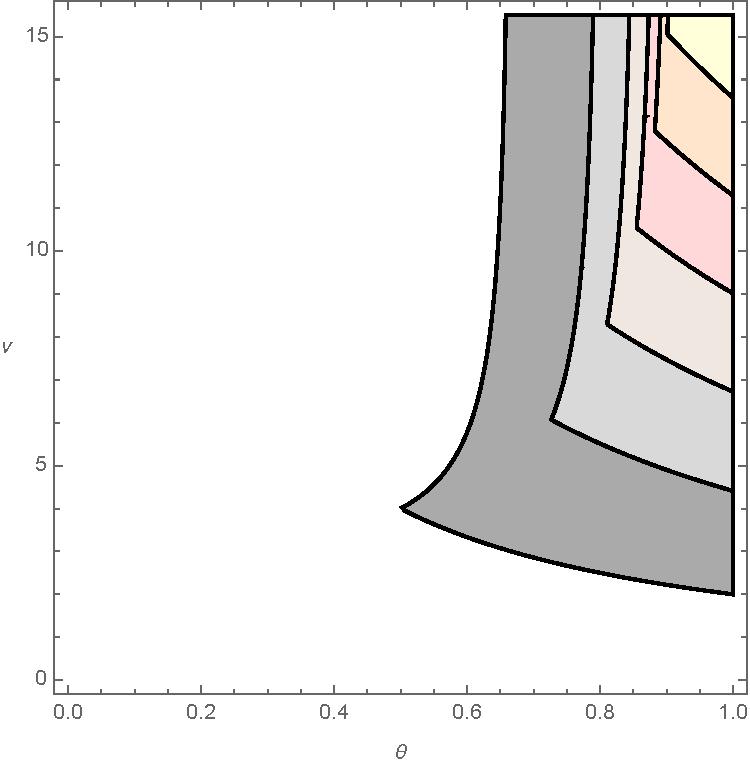
\includegraphics[width=0.48\textwidth]{fig_variousk.pdf}
\caption{The set of parameters ensuring $M(2k+1,\te,\nu)\ge 0$ in the $(\te,\nu)$ parameter plane}\label{fig_variousk}
\end{center}
\end{figure}

\begin{figure}
\begin{center}
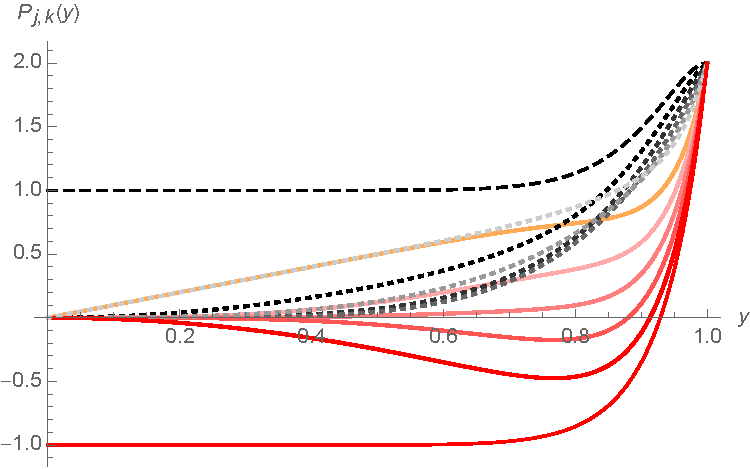
\includegraphics[width=0.5\textwidth]{fig_excepttopleft.pdf}
\caption{The polynomials in the first row of $M$, except the top left polynomial}\label{fig_excepttopleft}
\end{center}
\end{figure}

\begin{figure}
\begin{center}
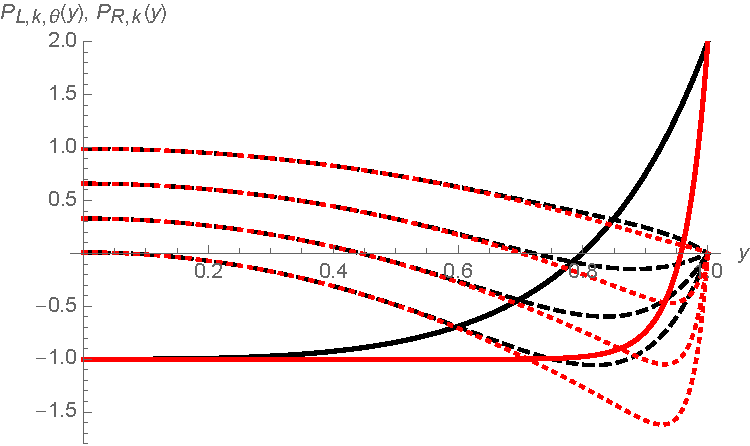
\includegraphics[width=0.5\textwidth]{fig_someplpr.pdf}
\caption{The red group ..., the black group ...}\label{fig_someplpr}
\end{center}
\end{figure}

\begin{figure}
\begin{center}
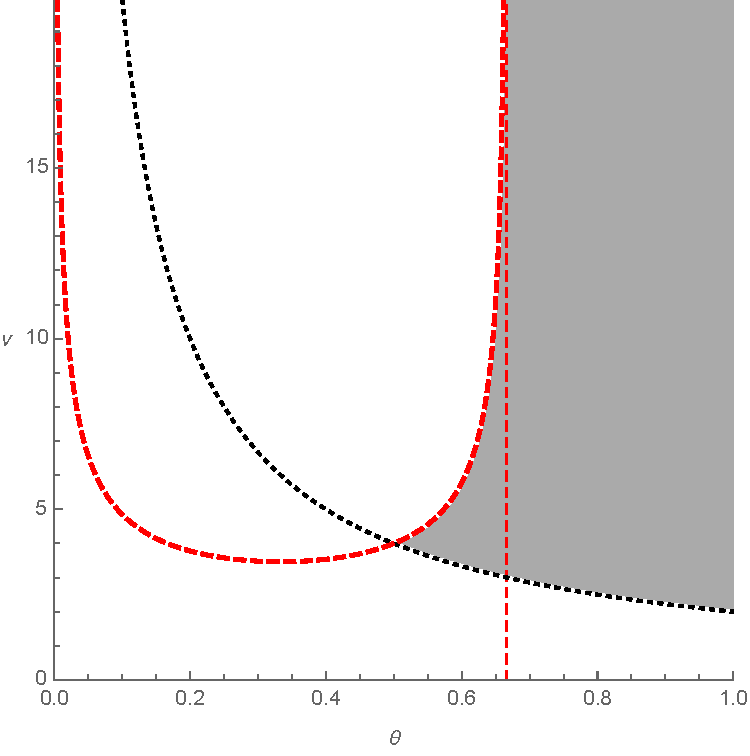
\includegraphics[width=0.48\textwidth]{fig_boundary.pdf}
\caption{Boundary curves for $m=3$ in the $(\te,\nu)$ parameter plane}\label{fig_boundary}
\end{center}
\end{figure}

... about the non-negativity of the top left, and the top right entries of $M$.
\begin{lemma}
For any $k\in\nplus$ and $\te\in(0,1]$ we have 
\[
M_{1,1}(2k+1,\te,\nu)\ge 0 \quad \Longleftrightarrow \quad \nu\le\nul
\] 
and
\[
M_{1,2k+1}(2k+1,\te,\nu)\ge 0 \quad \Longleftrightarrow \quad \nu\ge\nur.
\] 
\end{lemma}


... a necessary and sufficient condition for the non-negativity of the matrix $M$ for odd sizes.
\begin{lemma}
For any $k\in\nplus$ and $\te\in(0,1]$ we have 
\[
M(2k+1,\te,\nu)\ge 0 \quad \Longleftrightarrow \quad \nur\le\nu\le\nul.
\] 
\end{lemma}

... to explain Figure \ref{fig_variousk} we use the following result.
\begin{lemma}
For any $k\in\nplus$ and $\te\in\left(0,\frac{1}{2}\right)$ we have 
\[
 \nur>\nul.
\] 
\end{lemma}

\section{Other discretizations}

\end{document}
